\chapter{序論}
\label{introduction}

本研究では,惑星規模の分散システムのための試験環境の設計と構築を行う.

本章では,惑星規模の分散システムを定義し,本研究の背景である惑星規模の分散システムの発達とシステムの試験環境について概説する.
本研究の課題を明らかにした上で,目的を明確化し,目的を達するための仮説を示す.
最後に仮説を裏付けるための提案手法を示し,本研究の概要を示す.

\section{本研究の背景}
\label{introduction:background}

本節では,本研究の背景について述べる.

初めに,本研究が対象とする惑星規模の分散システムと試験環境について概説する.
分散システムについて概説した上で惑星規模の分散システムを定義し,惑星規模の分散システムの発達について述べる.
加えて,惑星規模の分散システムに求められる試験環境について説明する.

\subsection{惑星規模の分散システム}

本節では,本研究における惑星規模の分散システムを定義する.

分散システムは,複数の構成要素が組み合わさって動作するシステムである.
各構成要素は独立しており,互いに協調動作することによってシステム全体が成り立っている.

惑星規模の分散システムは,分散システムの中でも世界中に地理的に分散したコンピュータによって構成されるものと定義する.
惑星規模の分散システムの基盤技術としては,P2Pがあげられる.

P2Pは``Peer to Peer''の略記であり,中央集権的なサーバを必要とせず,各コンピュータが互いに対等な関係を築き協調動作することで成り立つシステムモデルまたはその技術自体を指す.
P2Pは,システム内に明確な役割分担と主従関係のあるクライアントサーバモデルとは対照的なシステムモデルである.
クライアントサーバモデルは中央主権的なシステムであり,通信において常にクライアントとサーバで一対一の関係が成り立つ.
クライアントはサーバに対し処理や情報を要求し,要求を受け取ったサーバは特定の処理を行なってクライアントへ返答する.
対してP2Pシステムでは,システムを構成する各コンピュータの役割は状況に応じて柔軟に変化し,通信において多対多の関係が成り立つ.
クライアントとして他のコンピュータに対し要求する場合もあれば,他のコンピュータからの要求に対して応答する場合もある.
クライアントサーバモデルに比べて,拡張性(スケーラビリティ)ならびに耐障害性において優れているのが特徴的である.

ビットコインの中核技術であるブロックチェーンは,P2Pシステムの一例である.
ブロックチェーンのようなP2Pシステムでは,地理的に分散することによるネットワークでの通信の遅延を考慮した上で協調動作可能であることを開発者は意識しなければならない.

\subsection{惑星規模の分散システムの発達}

2000年代初頭,Winny~\cite{Winny}やGnutella~\cite{Gnutella}といった惑星規模の分散システムが頭角を現した.
どちらのサービスもP2P技術を基盤としており,それまでシステムモデルとして一般的であったクライアントサーバモデルとは異なる形態を採用したことで注目が集まった.
P2P技術が研究分野で取り上げられる頻度も多くなり,サービスとしても今後一層幅を広げていくと思われたが,クライアントサーバモデルに置き換わるまでの隆盛はなく後退していった.
しかし,2008年にSatoshi NakamotoによりBitcoinのために開発されたブロックチェーン技術が登場することによって,再度P2P技術が脚光を浴びるようになり,開発や研究の勢いが再び盛んになってきている.

\subsection{試験環境}

試験環境とは,公の実稼働環境での運用をする前にシステム全体の試験を行うための環境である.
開発者が実際に開発を行う開発環境と公の実稼働環境では,環境の差異から動作の違いが生じ,開発環境で正常に動作していたものが公の実稼働環境に反映した途端動作しなくなるといった事象が度々発生する.
そのような事態を防ぐために開発環境と公の実稼働環境の間に試験環境を構築し,公の実稼働環境への適用前に試験環境にてシステム全体の試験をすることで予想外の障害が発生する可能性を低減できる.
惑星規模の分散システムにおいても,システムの不具合を早期に発見するために試験環境が必要である.

先に述べたように,惑星規模の分散システムでは地理的に分散することによるネットワークでの通信の遅延が発生する.
よってシステムの試験は,通信の遅延を考慮した上で正常に協調動作することを確認する必要があるため,試験環境は地理的に分散したサーバによって構成されたものでなければならない.

既存の惑星規模の分散システムの試験環境としては, PlanetLabやパブリッククラウドサービスの活用, BSafe.networkがあげられる.
PlanetLabは,ネットワークサービスの開発を支援する研究ネットワークであり,世界中の717地域1353のサーバを利用することができ,
パブリッククラウドサービスでは,リージョンと呼ばれるデータセンターの地域を指定することでサーバを分散配置することが可能である.
最後に,BSafe.networkは32の大学によって構成されるブロックチェーン技術の研究を行うためのネットワークであり,世界中の各大学が保有するサーバを用いて開発を行える.

\begin{figure}[htbp]
  \begin{center}
    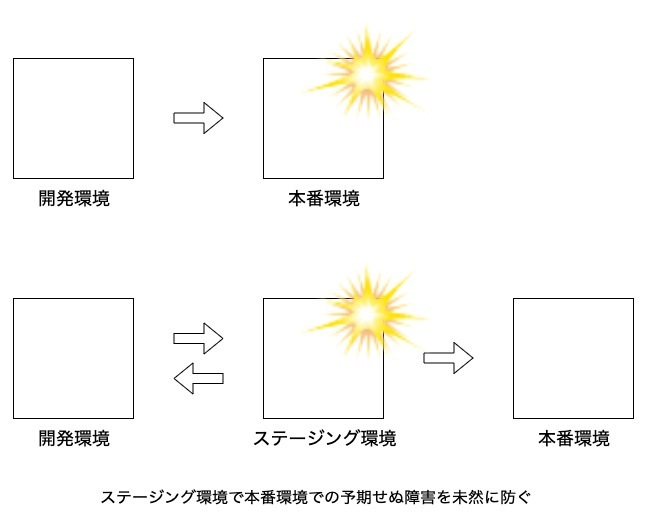
\includegraphics[width=0.8\textwidth]{./figures/staging.jpg}
    \caption{試験環境}
  \end{center}
\end{figure}

\section{本研究の課題と目的}
\label{introduction:issue-aim}

本節では,本研究の課題と目的を述べる.

まず,~\ref{introduction:background}章で述べた本研究の背景を元に,惑星規模の分散システムの試験環境における課題を示す.
その上で本研究の目的を明確にする.

\subsection{本研究の課題}
\label{introduction:issue-aim:issue}

本研究では,既存の惑星規模の分散システムの試験環境の課題について指摘する.

惑星規模の分散システムの試験では,地理的に分散配置されることによるネットワークでの通信の遅延を考慮した上で各コンピュータが正常に協調動作を行えるかを確認する必要があり,
試験環境では各サーバを実際に地理的に分散配置する必要性があることは~\ref{introduction:background}章の背景で述べた通りである.
さらに既存の試験環境として, Planet Labやパブリッククラウドサービスのリージョンの活用, BSafe.networkがあげられるが,それぞれ課題があると考える.
Planet Labでは世界中に分散したサーバを利用することが可能だが, OSやCPU,メモリなどのサーバの環境を柔軟に変更することができない.
パブリッククラウドサービスでは,サーバの環境を自由に変更可能であり,リージョンを活用して地理的に分散した場所にサーバを設置することができるが,
リージョンが限定的であり,公の実稼働環境に比べネットワークでの通信の遅延が少ないため,環境に差異が生じてしまう.
BSafe.networkでは,世界中の32の大学が保有するサーバを用いてシステムの実験を行えるが,各サーバの管理権限が各大学のオペレータに委ねれられているため,
大学間での共同研究を行う場合にオペレータの手作業が必要である.

本研究では,このように惑星規模の分散システムの試験環境の構築手法が整備されていないことを課題とする.

\subsection{本研究の目的}
\label{introduction:issue-aim:aim}

本研究では,惑星規模の分散システムのための試験環境の構築手法を提案することを目的とする.

\section{本研究の仮説}
\label{introduction:hypothesis}

~\ref{introduction:issue-aim:issue}章で述べた課題を解決するため,本研究では地理的に分散したサーバを統合管理可能な試験環境の構築が必要であると考えた.
惑星規模の分散システムの試験環境は,
\begin{itemize}
  \item OSやCPU, Memoryといったサーバ環境を柔軟に変更可能であること
  \item 公の実稼働環境を想定したネットワークでの通信の遅延を考慮できること
  \item 異なる管理権限下にある各サーバに対し統合的管理が可能であり,各オペレータの手作業を軽減できること
  \item 地理的に分散した各サーバに対し,統合的な操作が可能であること
\end{itemize}
の四点を満たさなければならない.

本研究では,上記の必要要件を満たすことで~\ref{introduction:issue-aim:issue}で述べた課題点を解決し,
~\ref{introduction:issue-aim:aim}で述べた惑星規模の分散システムの試験環境の構築手法の提案を達成できると考えた.

\section{本研究の手法}
\label{introduction:proposal}

本研究では,~\ref{introduction:hypothesis}章で述べた必要要件を満たすため,OpenVPNとKubernetesを組み合わせた惑星規模の分散システムの統合的試験環境を提案する.

Kubernetesはコンテナオーケストレーションツールであり,コンテナ化仮想技術によってコンテナ化されたアプリケーションのデプロイやスケーリングを自動化し,統合管理するためのシステムである.
Kubernetesでは複数のサーバでクラスタを構成しており,クラスタリングを行うためには各サーバが互いにIPレベルで疎通可能な状態になければならない.
よって,IPレベルでの疎通が取れない別々のセグメントに配置されたサーバ間ではKubernetesクラスタを構築することはできない.

そこで地理的に分散し異なるセグメントに配置されたサーバ間を繋ぐOpenVPNオーバーレイネットワークを構築することで,各サーバを互いにIPレベルで疎通可能にする.
OpenVPNは,VPNネットワークの構築をソフトウェアで実現するために開発されたオープンソースソフトウェアである.

本研究では, OpenVPNとKubernetesを組み合わせ,地理的に分散した拠点間で形成したOpenVPNオーバーレイネットワーク上でKubernetesクラスタを構築した.
本システムが本研究における課題点を解決できているか推定することで,要件を満たせることを確認した.

\section{本論文の構成}
\label{introduction:structure}

本論文における以降の構成は次の通りである.

~\ref{background}章では,惑星規模の分散システムと試験環境ならびに本研究で使用する技術について概説し,本研究の背景を明確化する.
~\ref{issue}章では,本研究における課題を明確化し,課題を解決するための要件,仮説と手法について概説する.
~\ref{implementation}章では,本研究で提案する試験環境の構築方法について述べる.
~\ref{evaluation}章では,\ref{issue}章で述べた課題に対しての評価を行い,考察する.
~\ref{conclusion}章では,本研究のまとめと今後の課題についてまとめる.

%%% Local Variables:
%%% mode: japanese-latex
%%% TeX-master: "../thesis"
%%% End:
